\documentclass[a4paper,10pt,twocolumn]{article}
\usepackage[a4paper,right=1.5cm,left=1.5cm,top=2cm,bottom=2.5cm,headsep=0cm,footskip=0.5cm]{geometry}
\usepackage[spanish,activeacute,es-tabla]{babel}

%\usepackage{multicol}
\usepackage[utf8]{inputenc}
\usepackage{enumitem}
\usepackage{amsmath}
\usepackage{times}
\usepackage{graphicx}
\usepackage{float}
\usepackage{csquotes} 
\usepackage{multirow}
\usepackage{xcolor}
\usepackage{colortbl}
\usepackage[colorlinks=true,allcolors=blue]{hyperref}
\usepackage{titlesec}

\setlength{\parindent}{0pt}
\setlength{\parskip}{6pt}
\setlength{\columnsep}{1cm}

\titleformat{\section}{\large\bfseries}{\thesection}{1em}{} % Cambia el tamaño de la fuente de las secciones a \large
\titleformat{\subsection}{\small\bfseries}{\thesubsection}{1em}{} % Cambia el tamaño de la fuente de las subsecciones a \large
\titleformat{\subsubsection}{\small\bfseries}{\thesubsubsection}{1em}{} % Cambia el tamaño de la fuente de las subsubsecciones a \large
\titlespacing{\section}{0pt}{\parskip}{\parskip}
\titlespacing{\subsection}{0pt}{\parskip}{\parskip}

\newcommand{\link}[1]{{\color{blue}\href{#1}{#1}}}
\renewcommand\thesection{\arabic{section}.}
\renewcommand\thesubsection{\arabic{section}.\arabic{subsection}.}

\title{\LARGE \textbf{Plantilla de las contribuciones al Congreso Anual de la Sociedad Española de Ingeniería Biomédica (CASEIB)}}

\author{\large N. ApellidosAutor1 $^1$, N. ApellidosAutor2 $^{1,2}$, N. ApellidosAutor3 $^{1,2,3}$
\\
\\
\small $^1$ Departamento, Universidad, Ciudad, País, \{email1, email2\}@dpto.univ.pais \\
\small $^2$ Servicio, Hospital, Ciudad, País, email@hosp.pais \\
\small $^3$ Afiliación3 \\
}
\date{} % Elimina la fecha

\pagestyle{empty}
\sloppy

\begin{document}	

\maketitle
\thispagestyle{empty}

\begin{center}
\large
\textbf{Resumen}
\end{center}
\small
\textit{Esta plantilla de muestra de \LaTeX\/ provee las pautas básicas para ayudarle a preparar los documentos a presentar. Los documentos se publicarán exactamente como sean recibidos. Para asegurar un aspecto profesional y una máxima uniformidad entre todos los documentos, le pedimos cordialmente que ponga mucha atención en respetar estas pautas básicas, las cuales indican las áreas típicamente disponibles para cada parte del documento, desde el título hasta el texto principal así como el tipo y tamaño de las fuentes sugerido. \textbf{La longitud máxima del resumen son 250 palabras}}. 

\normalsize

\section{Motivación}
Las pautas para la presentación de los documentos son un elemento importante para ayudar en la obtención de un aspecto profesional y una calidad aceptable. Son muy fáciles de seguir con los actuales procesadores de textos generalmente disponibles. Basta con tomar debida nota de las áreas que están típicamente disponibles para cada parte del documento así como el tipo y tamaño de las fuentes sugerido. Para verla mejor, esta plantilla de muestra está completamente escrita con las fuentes sugeridas para ser usadas en el documento. La puede conseguir en \link{https://caseib.es/2024}.

Si después de leer estas normas sigue teniendo alguna duda, el autor puede consultar por correo electrónico a \href{mailto:contacto@caseib.es}{contacto@caseib.es}.
 
\section{Márgenes, fuentes y espaciado entre líneas}
El documento debe tener como máximo \textbf{4 páginas de longitud}, y debe escribirse en \textbf{DIN-A4} (21 cm x 29,7 cm) con los siguientes márgenes:
\begin{itemize}[topsep=0pt, partopsep=0pt, parsep=0pt]
\item 2 cm, desde el margen superior hasta la primera línea en cada página.
\item 2,5 cm, desde el margen inferior hasta la última línea del texto.
\item 1,5 cm, hasta el margen interior del documento.
\item 1,5 cm, hasta el margen exterior del documento.
\item 0,5 cm de margen de encuadernación.
\end{itemize}

Los márgenes del documento deberán ser simétricos. Recordar que la primera página de la contribución será numerada posteriormente como impar.

El título, nombres de los autores y sus datos deben ser escritos en formato de una columna y centrados en la parte superior de la primera página, mientras que el resto del texto debe hacerse en formato de 2 columnas con alineación justificada. El espacio entre columnas es 1 cm, lo que deja 8,25 cm para el ancho de cada columna, exactamente como está formateada esta plantilla. Se debe evitar dividir palabras.

La fuente sugerida para usarse en el documento es Times New Roman. A continuación puede encontrar el autor una relación de los tamaños de letra y espaciados de párrafo en función de la importancia de la parte del documento escrita:
\begin{itemize}[topsep=0pt, partopsep=0pt, parsep=0pt]
\item Para el título de la contribución sugerimos Times New Roman 18 negrita y un espaciado posterior de 24 puntos.
\item Los nombres y datos de los autores se sugieren en Times New Roman 12 y 10 respectivamente y los espaciados posteriores serán de 12 y 4 puntos.
\item El resumen seguirá una fuente Times New Roman 9 itálica con espaciado posterior de 12 puntos.
\item El cuerpo principal del documento estará en Times New Roman 10 con espaciado posterior de 6 puntos.
\item Los encabezamientos de sección en Times New Roman 12 negrita y espaciados anterior y posterior de 6 puntos.
\item Para las referencias se recomienda Times New Roman 9 con espaciado posterior de 6.
\item Los pies de figuras, tablas y ecuaciones pueden formatearse con Times New Roman 9 itálica. Los espaciados anterior y posterior, serán de 6 puntos.
\end{itemize}

En relación con el espaciado en el formato de párrafo hay dos reglas sencillas: el interlineado debe ser sencillo y el espaciado posterior debe ser 6 puntos tal y como está formateado este documento.

\section{Secciones}
Además del título y los nombres y datos de los autores, la primera página contiene el resumen. Debido a su importancia en la estructura global del documento, aparece en la parte superior de la primera columna y no debe ocupar más de 15 líneas de texto.

A continuación aparecerá el desarrollo de las distintas secciones en las que está organizado el documento. Los títulos de las secciones, por ejemplo: ``1. Introducción'', deben aparecer en negrita y alineados a la izquierda, con una tabulación y sangría de 0,76 cm. Utilice un punto y no un guion después del número.

\subsection{Subsecciones}
Los títulos de las subsecciones deben estar en minúsculas (excepto la letra inicial) y en negrita. Deben empezar a la izquierda, en una nueva línea, y con una tabulación y sangría de 1,02 cm. 

No se aconseja utilizar niveles inferiores al de subsecciones, pero si son imprescindibles, deben aparecer en minúsculas (excepto la primera letra) y en itálica, y deben comenzar a la izquierda en una línea nueva.

\section{Encabezados, notas y pies de página}
Por favor, \textbf{no} ponga encabezado o pie de página, ni incluya números de página. Éstos se insertarán posteriormente cuando se incluya la comunicación en el libro de actas. 

Evite las notas a pie de página (por ejemplo, poniéndolas entre paréntesis). Si no es posible evitarlas, sitúelas en la misma columna en la que está la referencia.

\section{Acerca de las figuras}
Siempre que sea posible, se sugiere colocar las figuras lo más cerca del lugar del texto donde se les haga referencia por primera vez (como en la Figura~1). 

\begin{figure}[hbt]
	\centering
	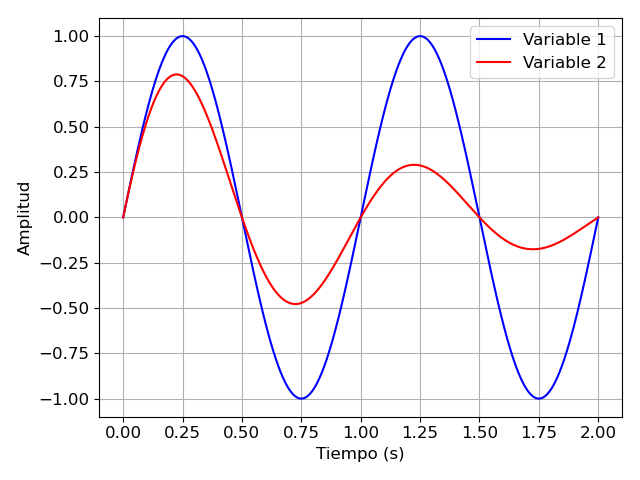
\includegraphics[width=\columnwidth]{figura.png}
	\textit{\textbf{Figura 1.} Ejemplo de pie de figura}
	\label{Figura1}
\end{figure}

Para evitar que las imágenes se descoloquen durante la edición del libro de actas, su estilo de ajuste deberá ser ``en línea con el texto''. Por otra parte, la figura se centrará y se procurará adecuar su tamaño para que ocupe la anchura de una columna. En caso de que sea necesario emplear las dos columnas, el ancho no podrá superar un máximo de 17,5 cm. Para que la figura se visualice correctamente, se recomienda utilizar una resolución mínima de 300 dpi.

Los pies de las figuras deben ir escritos justo debajo de la figura, preferiblemente centrados con referencia a la misma. Las figuras se numeran secuencialmente y el número de orden, así como la palabra Figura, deberán ir en negrita seguidas de un punto.

\section{Acerca de las tablas y bibliografía}
Para las tablas se puede usar negrita y diferentes tamaños (desde Times New Roman 10 hasta 8 puntos) para diferenciar la información relevante que contienen. Respecto a su anchura y formato del pie, las pautas a seguir serán las mismas que en el caso de las figuras.

\begin{center}
\begin{tabular}[hbt]{c c c c}
	\label{Tabla1}
	Distorsión & 2 Arm. & 3 Arm. & 4 Arm. \\
	\hline
	\hline
	\textit{Señal A} & -51 dB & -53 dB & -51 dB \\
	\textit{Señal B} &	-76 dB & -65 dB & -76 (dB) \\
	\hline
	\hline
\end{tabular}
\end{center}
\begin{center}
	\textit{\textbf{Tabla 1.} Ejemplo de pie de tabla}
\end{center}

Enumere las referencias bibliográficas, por orden de aparición, al final de la comunicación. Al referirse a ellas en el texto, escriba el número correspondiente entre corchetes: \cite{Bigio_2016} si se trata de un libro, \cite{Shariat_2024} si es un artículo, \cite{Romitti_2022} si es una comunicación en un congreso, y \cite{caseib_2024} si es una referencia a un recurso en Internet. En caso de múltiples referencias, separarlas por una coma \cite{Bigio_2016,Romitti_2022} o un guion en el medio \cite{Bigio_2016,Shariat_2024,Romitti_2022} si se trata de referencias consecutivas.

\section*{Agradecimientos}
Agradecemos a los anteriores comités organizadores del CASEIB su amabilidad al permitirnos usar sus guías de estilo como referencia.

% ---- Bibliography ----
\begin{small}
\bibliographystyle{ieeetr}
\bibliography{references}
\end{small}

\end{document}
